%---------------------导言区---------------------------%
\documentclass[12pt,a4paper,UTF8]{ctexart}
	%10pt:正文字体为12pt,缺省为10pt;各层级字体大小会根据正文字体自动调整
	%a4paper:纸张大小a4;
	%UTF8:中文要求
%\usepackage{syntonly}
%\syntaxonly%加快编译速度
\usepackage{geometry}%用于设置上下左右页边距
	\geometry{left=2.5cm,right=2.5cm,top=3.2cm,bottom=2.8cm}
\usepackage{multirow}
\usepackage{xeCJK,amsmath,paralist,enumerate,booktabs,multirow,graphicx,float,subfig,setspace,listings,lastpage,hyperref,gensymb}
	%xeCJK:中文字体(如楷体,作者和机构需要用到)的设置
	%amsmath:数学公式
	%paralist,enumerate:自定义项目符号
	%booktabs:三线图,论文常用的表格风格
	%multirow:复杂表格
	%graphicx,float: 插入图片
	%subfig:并排排版图片以及强制图表显示在“这里”[H]
	%setspace:设置行间距等功能
	\setlength{\parindent}{2em}%正文首行缩进两个汉字
	%listings:用于排版各种代码;比如matlab的代码
	%\lstset{language=Matlab}%matlab代码
	%lastpage:获取总页数;
	%hyperref:超链接,和lastpage搭配.
\usepackage{fancyhdr}
	%fancyhdr:一个很强大的宏包,用于自定义设计页面风格并命名以供调用。
	\pagestyle{fancy}
	\rhead{实验十五~非平衡电桥测量铂电阻的温度系数}
	\lhead{普通物理实验\uppercase\expandafter{\romannumeral1}实验报告}
	\cfoot{\thepage}  
		%分别是右页眉、左页眉、右页脚
	\renewcommand{\headrulewidth}{0.4pt}
	\renewcommand{\theenumi}{(\arabic{enumi})}

\setCJKmainfont{FZSSK.TTF}[ItalicFont=FZKTK.TTF, BoldFont=FZHTK.TTF]
%中文字体设置:使用开源字体方正书宋,方正楷体和方正黑体



%%%%%%%%%%%%%%%%%%%%%%%%%%%%%%%%%%%%%%%%%%%%%%%%%%%%%%%%%%
%%%%%%%%%%%%%%%%%%%%%%%%%正文开始%%%%%%%%%%%%%%%%%%%%%%%%%%
%%%%%%%%%%%%%%%%%%%%%%%%%%%%%%%%%%%%%%%%%%%%%%%%%%%%%%%%%%

\begin{document}

%%begin-------------------标题与信息-----------------------%%

%%标题
\begin{center}
\LARGE\textbf{实验十五~非平衡电桥测量铂电阻的温度系数}
\end{center}

%%信息
\begin{doublespacing}
	%doublespacing:手动两倍行距
	\centering
	\begin{tabular}{ll}
	 & \\
	{\CJKfontspec{STKAITI.TTF} 实验人:钟易轩}  & {\CJKfontspec{STKAITI.TTF}指导教师:张晓东}\\
	{\CJKfontspec{STKAITI.TTF} 组号:九组七号} & {\CJKfontspec{STKAITI.TTF}学号:2000012706}\\
	{\CJKfontspec{STKAITI.TTF} 实验时间:2021年11月26日} &{\CJKfontspec{STKAITI.TTF} 实验地点:物理楼南楼~233}
	\end{tabular}
\end{doublespacing}

%%end-------------------标题与信息-----------------------%%
\subsection*{【实验目的】}
\begin{enumerate}[(1)]
\item 了解铂电阻传感器的温度特性;
\item 了解电阻的三线接法;
\item 测定铂电阻的温度系数.
\end{enumerate}
\subsection*{【仪器用具】}
$ZX96$型电阻器,数字温度计,$VC9806$型数字万用表,恒流源,电加热杯,冰水混合物,开关,导线.\par
\begin{table}[htbp]
\centering
\caption{$ZX96$型直流电阻器允差}
\begin{tabular}{|c|c|c|c|c|c|c|}
\hline
\textbf{挡位($\Omega$)}&$\times10k\Omega$&$\times 1k\Omega$&$\times100\Omega$&$\times10\Omega$&$\times1\Omega$&$\times0.1\Omega$ \\
\hline
\textbf{允差$e$}&$\pm0.1\%$&$\pm0.1\%$&$\pm0.1\%$&$\pm0.1\%$&$\pm0.5\%$&$\pm2\%$ \\
\hline
\end{tabular}
\end{table}
\par
$VC9806$型数字万用表的允差为:\par
$20mA$档允差:$0.5\%\times$读数+$0.004mA$;\par
$200mV$档允差:$0.05\%\times$读数+$0.03mV$.
\subsection*{【数据处理】}
在非平衡电桥实验中,主要是测定$U_{out}$与$T$的关系,如(15.1)式.
\begin{equation}
U_{out}=\frac{I_0}{2}R_0A_1\Delta T    \tag{15.1}
\end{equation}
\par
根据(15.1)式,测量不同温度时的$U_{out}$,得到表2.
\newpage
在$T=-0.1^{\circ}C$时,调整$R_p$的值,当$R_p=100.0(\Omega)=R_0$时,$U_{out}=0.05(V)$.同时也记录下此时的$I_0=4.001mA$.
\begin{table}[htbp]
\centering
\caption{$U_{out}$与$T$对应表}
\begin{tabular}{cccccccc}
\toprule
$T/^{\circ}C$&-0.1&23.6&40.6&55.3&70.1&85.1&100.7 \\
\hline
$U_{out}/mV$&0.05&18.16&31.08&42.34&53.45&64.75&76.42 \\
\bottomrule
\end{tabular}
\end{table}
\par
根据表2中数据,画出线性回归图.
\begin{figure}[htbp]
		\centering
		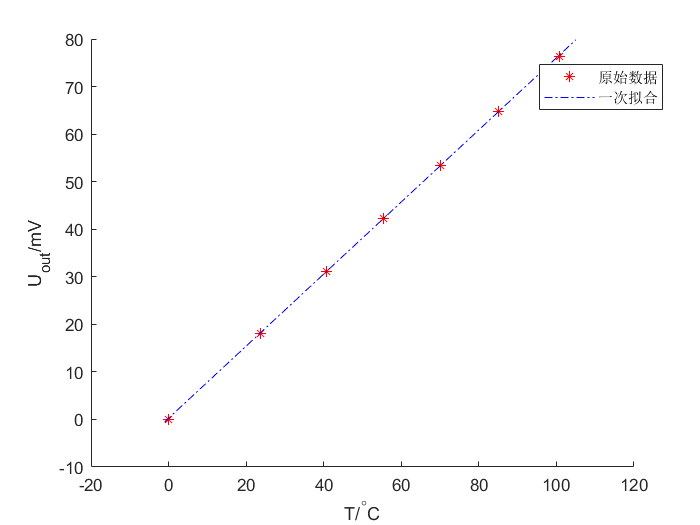
\includegraphics[width=9cm]{huigui.png}
		\caption{$U_{out}$与$T$线性回归图}
	\end{figure}
\par
因此求得相关系数为$r=0.9999908$,斜率为$k=0.7579(mV/^{\circ}C)$,温度系数$A_1=3.79\times10^{-3}(/^{\circ}C)$.再计算温度系数的不确定度,公式为
\begin{equation}
\sigma_{A_1}=A_1[(\frac{\sigma_k}{k})^2+(\frac{\sigma_{I_0}}{I_0})^2+(\frac{\sigma_{R_0}}{R_0})^2]^{\frac{1}{2}} \tag{15.2}
\end{equation}
\par
再由$VC9806$数字万用表的允差以及$ZX96$型直流电阻器的允差可得:
\begin{align*}
\sigma_{I_0}&=\frac{1}{\sqrt{3}}\times(0.5\%\times4.001+0.004)\approx \frac{1}{\sqrt{3}}\times0.024(mA) \\
\sigma_{R_0}&=\frac{1}{\sqrt{3}}\times(100\times0.1\%)=\frac{1}{\sqrt{3}}\times0.1(\Omega)
\end{align*}
\par
再计算$\sigma_k$的值,由于$\sigma_k=\sqrt{\sigma_{k_{fit}}^2+\sigma_{k_U}^2+\sigma_{k_T}^2}$,其中由拟合造成的不确定度为
\begin{equation*}
\sigma_{k_{fit}}=k\sqrt{\frac{1/r^2-1}{7-2}}=1.45\times10^{-3}(mV/^{\circ}C)
\end{equation*}
\par
现计算由横纵坐标$T$与$U_{out}$造成的不确定度.\par
首先最大电压的允差为$e_U=0.05\%\times 76.42+0.03=0.06821(mV)$,温度的允差用分度值代替,即$e_T=0.1^{\circ}C$.则有
\begin{align*}
\sigma_{k_U}=\frac{e_U/\sqrt{3}}{\sqrt{\sum_{i=1}^7(T_i-\bar T)^2}}=4.6\times10^{-4}(mV/^{\circ}C)\\
\sigma_{k_T}=\frac{ke_T/\sqrt{3}}{\sqrt{\sum_{i=1}^7(T_i-\bar T)^2}}=5.1\times10^{-4}(mV/^{\circ}C)
\end{align*}
\par
最后带入以上数据,算出$\sigma_{A_1}=1.56\times10^{-5}(/^{\circ}C)$,则有$A_1=(3.79\pm0.02)\times10^{-3}/^{\circ}C$.
\subsection*{【思考题】}
\begin{enumerate}[(1)]
\item 实验中有哪些因素会引起输出-输入非线性误差?对测量的影响有多大?本实验采取了什么措施,用以改善非平衡电桥的线性? \\
答:公式(15.1)是一个近似公式,需要$R_1 \gg R_T$,$R_2 \gg R_P$,如果这个条件不满足那么非线性就会加强,其次一些温度、磁场的改变以及导线的电阻干扰等都会影响线性.因此本实验采取了$R_1$和$R_2$远大于100$\Omega$,使用三线接法以及线性拟合等措施来改善非平衡电桥的线性.
\item 处理实验数据时,如果发现$U_{out}-T$拟合直线截距不为零,是何原因?这是否会影响测温精度? \\
答:由于第一个数据$T=-0.1^{\circ}C$时,$U_{out}>0$,那么在拟合中,直线截距就不是零了.但是应该不会影响测温精度.
\end{enumerate}
\subsection*{【分析与讨论】}
铂电阻的温度系数测量结果为$A_1=(3.79\pm0.02)\times10^{-3}/^{\circ}C$,而理论值为$A_1=3.85\times10^{-3}/^{\circ}C$.因此测量值是小于理论值的,其原因是在温度升高时,由于电阻的变化,导致电桥两臂的电流不再相等,从而导致测量值的减小.


\end{document}